\section{Acceleration}
Acceleration is a class implemented to represent the $Acc$ node from the Bayesian network. It inherits from the abstract Variable class, where the Variable class serves as a structure that all nodes in the network must have.

Since Acceleration inherits from Variable it has to implement two methods, \lstinline$UpdateVariance$ and \lstinline$UpdateMean$.
The mean value is the accelerometer reading.
The variance for the acceleration is a constant value and is determined by testing, which is described in \secref{section:finding-the-variance}.
Furthermore, when inheriting from Variable a matrix multiplication method is provided, as well as four properties, keeping track of a stochastic variable's mean, variance, and its parents.

The readings from the accelerometer were uncertain, as of such, the variance for the accelerometer readings was determined, which is described hereafter.

\subsection{Finding the Variance}\label{section:finding-the-variance}
To measure the distribution of noise from the accelerometer, the formula for finding variance, as shown in \secref{section:normal-distribution}, will be utilised.
The device was placed on a flat surface for a period of three minutes, to record a set of accelerations containing noise.
This data was used to calculate $\mu$, which is the mean value for the stochastic variable $X$.
The expected value would be zero, as the device was not in motion when the data was recorded.
The following formula was used to approximate the mean acceleration:

\begin{equation*}
\mu = \frac{1}{n}\sum\limits_{i=1}^n\left(X_i\right)
\end{equation*}
 	
where, $n$ is the amount of data entries and $X_i$ is the $i$'th entry.
For the chosen device, the mean value was calculated to $\textbf{0.00026 g}$.
When the mean value is known, it can be used to approximate $\sigma^2$, which is the variance which can be approximated as follows:

\begin{equation*}
\sigma^2 = \frac{1}{n}\sum\limits_{i=1}^{n}\left( X_i - \mu \right)^2
\end{equation*}

where, $n$ is the amount of data entries, $X_i$ is the $i$'th entry, and $\mu$ is the mean value.
For the chosen device, the variance was calculated to $\textbf{0.00552 g}$.

By finding the mean value and the variance, a normal distribution can be implemented on measured accelerations by using the \eqref{eq:normaldist} as repeated below:

\begin{equation*}
f(x) = \frac{1}{\sigma \sqrt{2\pi}}e^{-\frac{(x - \mu)^2}{2 * \sigma^2}}
\end{equation*}

\figref{fig:finding-the-variance-chart} shows the final result of finding the normal distribution.
The red points plotted in the graph, is the amount of times the specific value has been recorded during the three minutes of recording.
The blue graph shows the normal distribution which has been calculated from the recorded values.
It can be seen that the red points and blue graph are not aligned.
However, it is not an issue, since the ordinate axis specifies amount and density for the red points and blue graph respectively.

\begin{figure}[h]
\centering
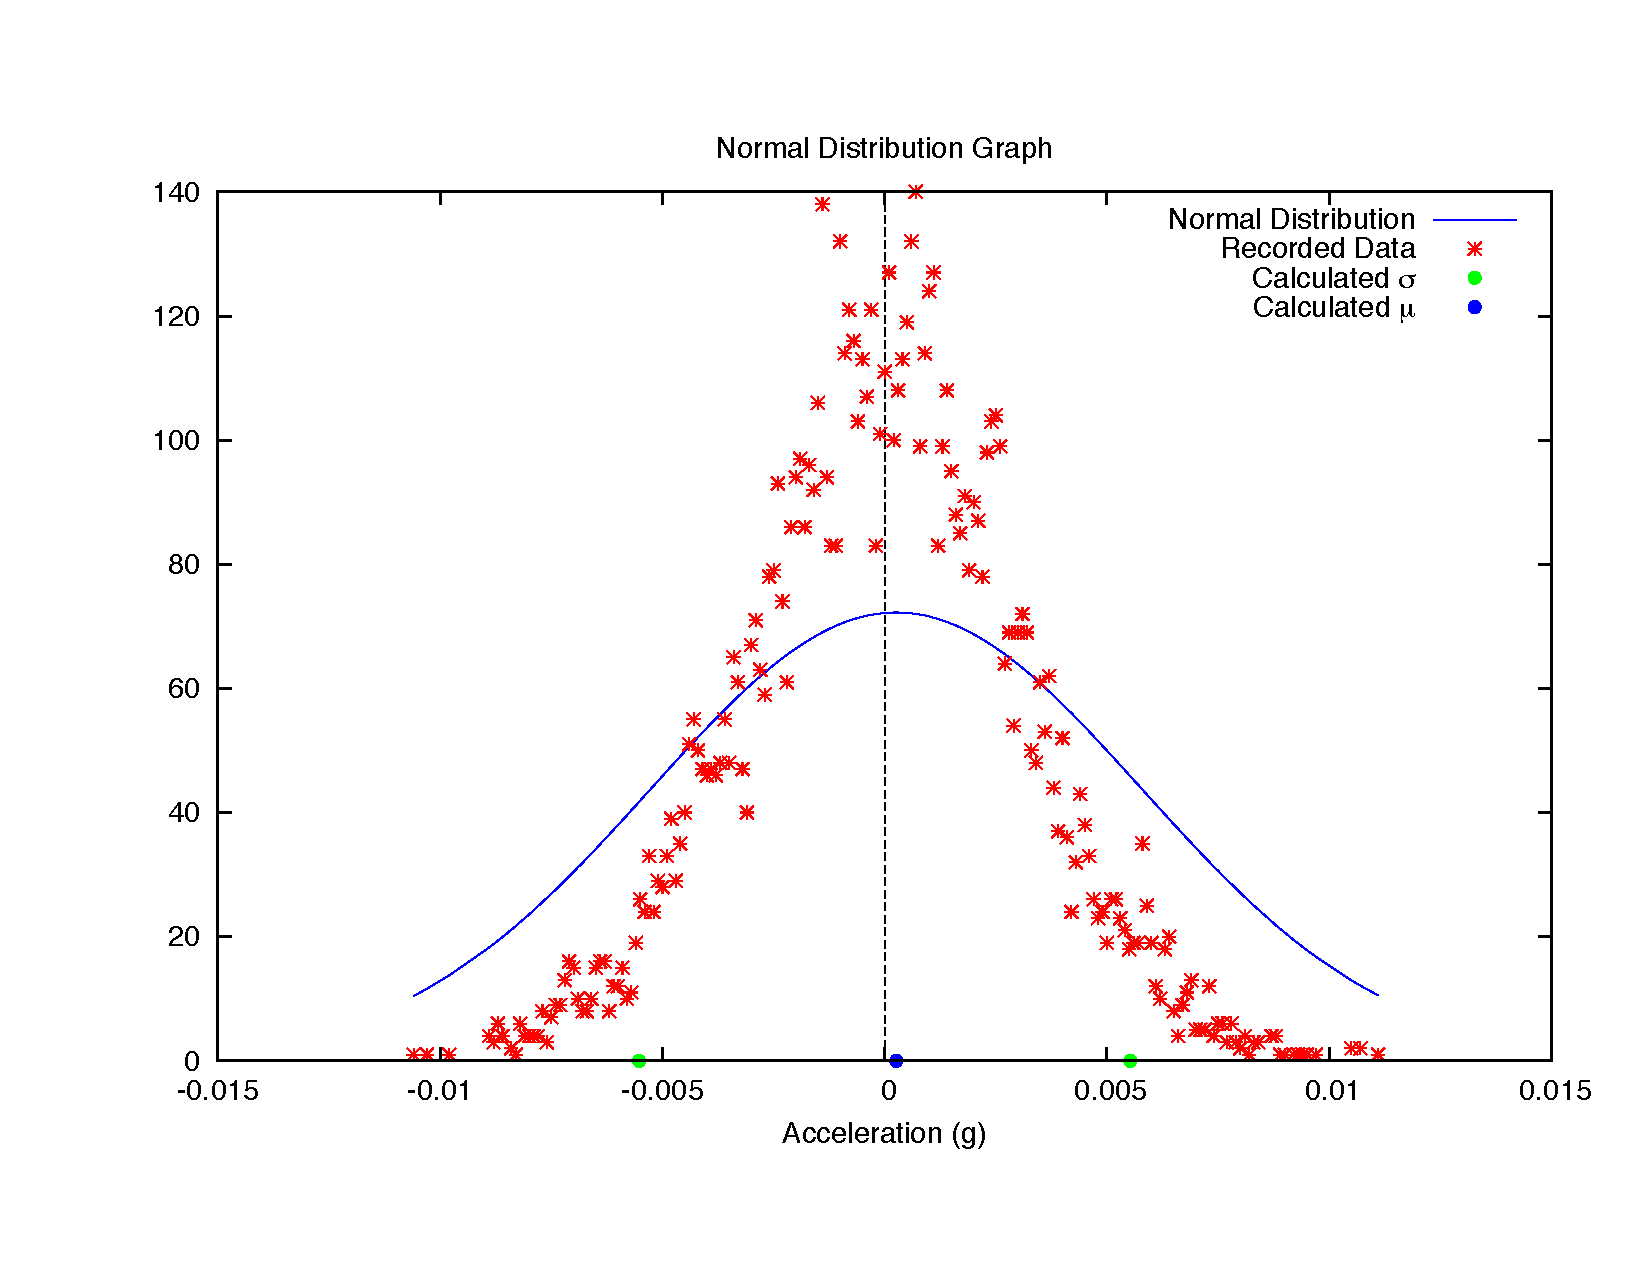
\includegraphics[trim = 0cm 2cm 0cm 2cm, clip, scale=0.45]{media/gnuplot/normaldist.pdf}
\caption{Finding $\mu$, $\sigma$, and the normal distribution}
\label{fig:finding-the-variance-chart}
\end{figure}
